\documentclass[a4paper,11pt]{article}

\usepackage{préambule}

% théorème qui souligne son titre.
\newtheoremstyle{etape_style}
	{\topsep} % espace avant
	{2\topsep} % espace apres
	{} % Police utilisee par le style de thm
	{} % Indentation (vide = aucune, \parindent = indentation paragraphe)
	{\bfseries}% Police du titre de thm
	{.} % Signe de ponctuation apres le titre du thm
	{ }% Espace apres le titre du thm (\newline = linebreak)
	{\myuline{\thmname{#1}\thmnumber{ #2}\thmnote{ \normalfont{\textbf{#3}}}}}% composants du titre du thm : \thmname = nom du thm, \thmnumber = numéro du thm, \thmnote = sous-titre du thm

\theoremstyle{etape_style}
\newtheorem{etape}{Étape}
\newtheorem*{etape*}{Étape}

\addtolength{\topmargin}{-1cm}
\addtolength{\textheight}{1cm}

\title{Faire un jeu de course en Scratch}
\date{}
\author{}

\begin{document}

\maketitle

Le but est de faire un jeu de course simple sur Scratch. On pourra bouger un véhicule, et il faudra le faire aller jusqu'à la ligne d'arrivée.

\begin{greybox}[frametitle={Dessins}]
	On commence par faire les dessins !

	Il nous faudra :
	\begin{itemize}
		\item 3 \textit{arrière-plans} : Un pour la course, un si on gagne et un si on perd.
		\item 1 \textit{véhicule} : ça peut être n'importe quoi, mais il faut qu'il rentre sur la route !
	\end{itemize}
\end{greybox}

\begin{center}
	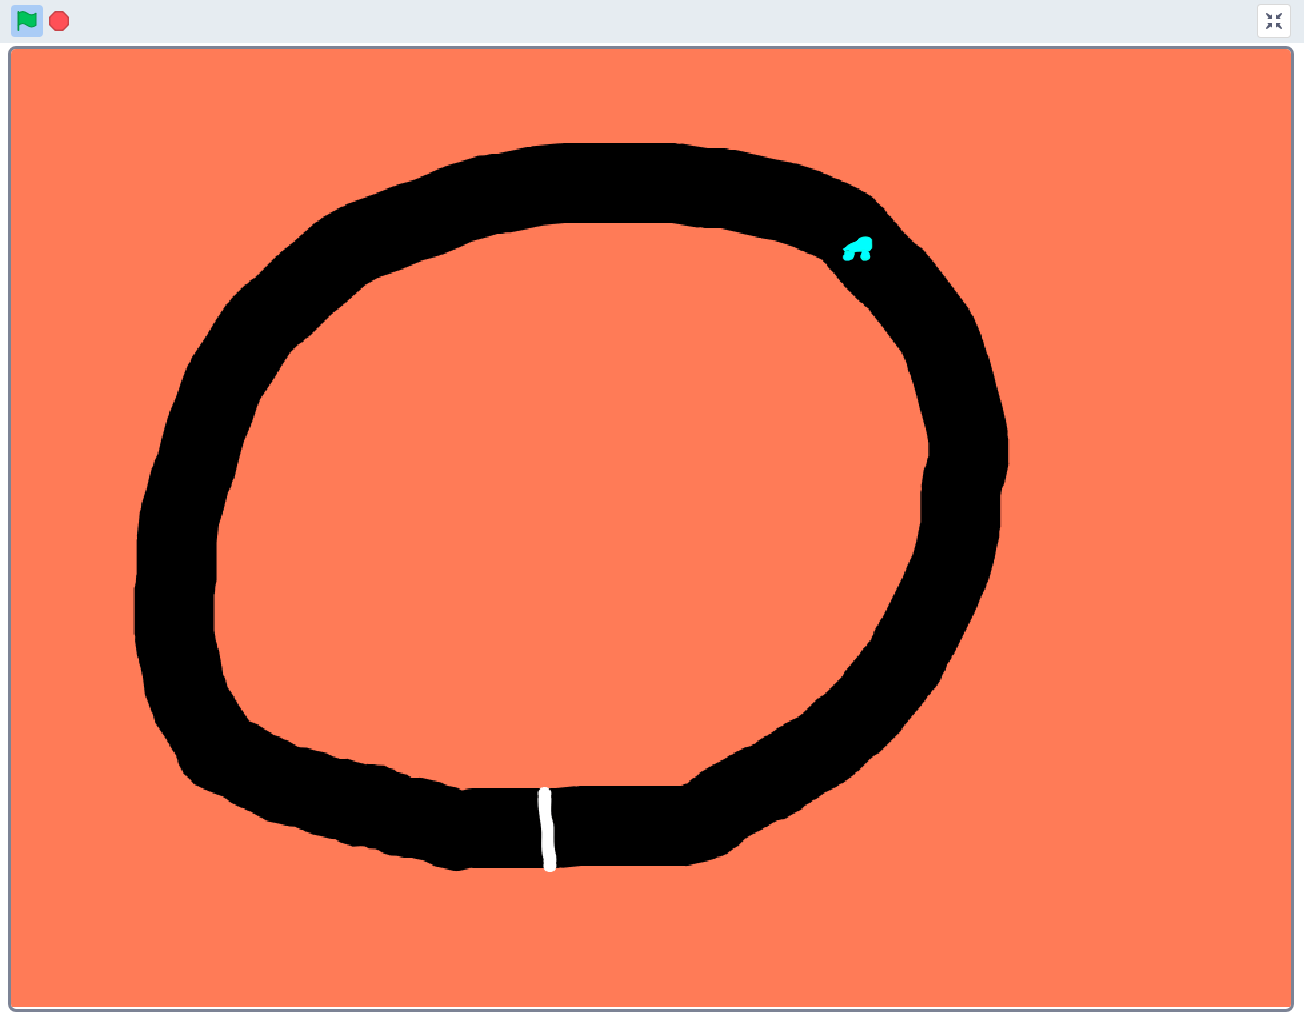
\includegraphics[width=0.3\textwidth]{Scratch-Course.png}
	\includegraphics[width=0.3\textwidth]{Scratch-Course-gagné.png}
	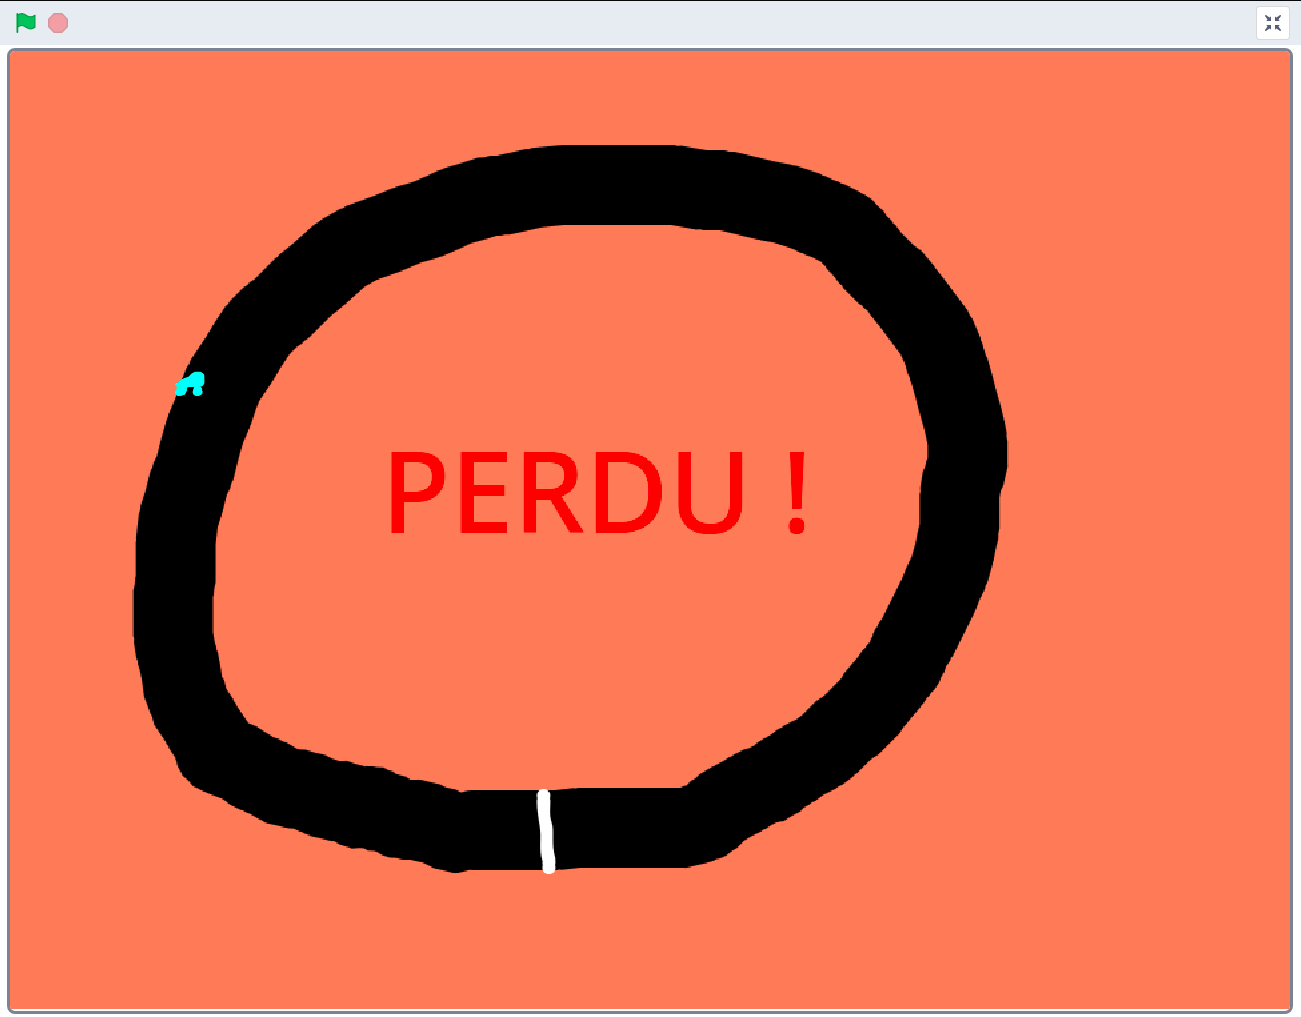
\includegraphics[width=0.3\textwidth]{Scratch-Course-perdu.png}
\end{center}

\begin{greybox}[frametitle={Règles}]
	\begin{itemize}
		\item Le véhicule commence sur la piste, et doit franchir la ligne d'arrivée.
		\item Le véhicule ne doit pas toucher le bords de la piste.
		\item On contrôle le véhicule avec le clavier ou la souris.
	\end{itemize}
\end{greybox}

\begin{etape}[: Placement initial]
	On voudrais que le jeu démarre lorqu'on appuie sur le drapeau.

	Arrange les blocks pour que le véhicule se mette à la position de départ lorqu'on appuie sur le drapeau.

	Pour cela, il faut utiliser des blocks de type \textit{Mouvement}.
\end{etape}

\begin{etape}[: Déplacement]
	Fait en sorte que le véhicule aille vers la droite lorsqu'on appuie sur la flèche de droite.

	\begin{palebox}[frametitle={\textit{Indice} :}]
		Regarde dans les catégories de blocks \textit{Évènements} ou \textit{Capteurs}.
	\end{palebox}

	Ajoute les autres directions.
\end{etape}

\begin{etape}[: Collisions]
	Si le véhicule atteint la ligne d'arrivée, on a gagné, et il faut afficher l'arrière-plan de victoire.

	Pour cela, tu peux utiliser les blocks \textit{Contrôle} → \squared{Si \_ alors}, et \textit{Capteurs} → \squared{Couleur \_ touchée ?}. \vspace{1em}

	On doit ensuite faire en sorte que le joueur ai perdu si on touche les bords de la piste.
\end{etape}

\begin{etape*}[Bonus]\

	\begin{itemize}
		\item Faire en sorte que le véhicule soit toujours tourné dans la direction où il va.
		\item Faire un chronomètre.
		\item Introduire un deuxième véhicule, qui fait la course tout seul 😨 !
	\end{itemize}
\end{etape*}

\end{document}